

\begin{frame}
\frametitle{Komunikacja międzyprocesowa}
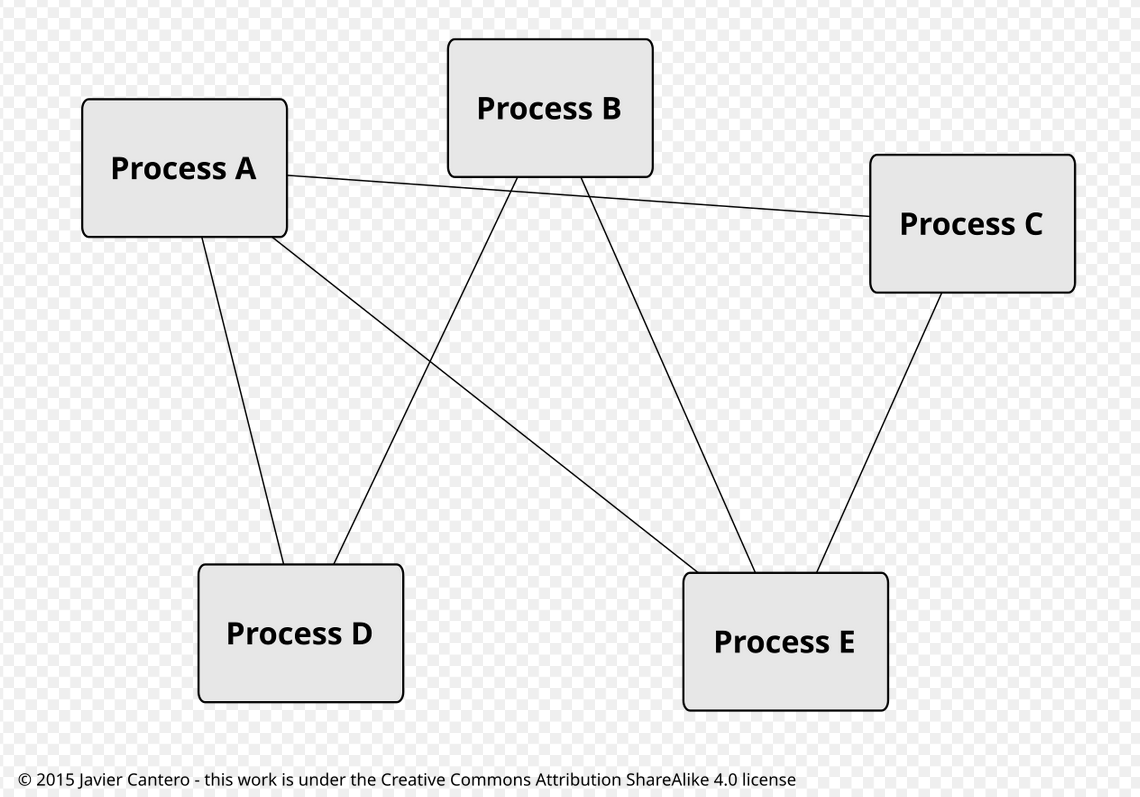
\includegraphics[width=\textwidth,height=\textheight,keepaspectratio]{ipc.png}
\end{frame}

\begin{frame}
    \frametitle{Przykłady}
        \begin{itemize}
        \item Pamięć współdzielona
        \item Sockety
        \item Pipe, named pipe
    \end{itemize}
\end{frame}

\begin{frame}
    \frametitle{Wysokopoziomowe rozwiązania}
    \begin{itemize}
        \item CORBA, Common Object Request Broker Architecture
        \begin{itemize}
            \item Skomplikowany, złożony standard
            \item Transparentność lokacji
            \item Kompatybilność
        \end{itemize}
        \item DCOP, Desktop COmmunication Protocol
        \begin{itemize}
            \item Część KDE...
            \item ...do czasu D-Busa, KDE 4
        \end{itemize}
    \end{itemize}

\end{frame}


\begin{frame}
    \frametitle{freedesktop.org}
    Projekt z 2002 roku zarządzający między innymi:
    \begin{itemize}
        \item PulseAudio
        \item systemd
        \item Wayland
        \item Mesa
    \end{itemize}

\end{frame}
    


